
\documentclass[paper=a4, fontsize=11pt]{scrartcl}
\usepackage[T1]{fontenc}
\usepackage{fourier}

\usepackage[english]{babel}															% English language/hyphenation
\usepackage[protrusion=true,expansion=true]{microtype}	
\usepackage{amsmath,amsfonts,amsthm} % Math packages
\usepackage[pdftex]{graphicx}	
\usepackage{url}
\usepackage[margin=1in]{geometry}
\usepackage{float}
\usepackage{listings}

\lstset{
  aboveskip=3mm,
  belowskip=3mm,
  frame=single,
  tabsize=2
}

%%% Custom sectioning
\usepackage{sectsty}
\allsectionsfont{\centering \normalfont\scshape}

%%% Custom headers/footers (fancyhdr package)
\usepackage{fancyhdr}
\pagestyle{fancyplain}
\fancyhead{}											% No page header
\fancyfoot[L]{}											% Empty 
\fancyfoot[C]{}											% Empty
\fancyfoot[R]{\thepage}									% Pagenumbering
\renewcommand{\headrulewidth}{0pt}			% Remove header underlines
\renewcommand{\footrulewidth}{0pt}				% Remove footer underlines
\setlength{\headheight}{10pt}
\setlength{\headsep}{10pt}
\setlength{\textheight}{700pt}
\setlength{\footskip}{50pt}

%%% Equation and float numbering
\numberwithin{equation}{section}		% Equationnumbering: section.eq#
\numberwithin{figure}{section}			% Figurenumbering: section.fig#
\numberwithin{table}{section}				% Tablenumbering: section.tab#


%%% Maketitle metadata
\newcommand{\horrule}[1]{\rule{\linewidth}{#1}} 	% Horizontal rule

\title{
		\vspace{-3ex}
		\usefont{OT1}{bch}{b}{n}
		\normalfont \normalsize \textsc{School of Computer Science} \\ [25pt]
		\horrule{0.5pt} \\[0.4cm]
		\huge Tiny: Tracking People using Multiple Kinects \\
		\horrule{2pt} \\[0.5cm]
		\vspace{-2ex}
}
\author{
		\normalfont 								\normalsize
        Chi-Jui Wu\\[-3pt]		\normalsize
        \today
}
\date{}

\begin{document}
\maketitle

\section{Project}

Realtime people detection and tracking are essential aspects of surveillance, medical monitoring, personalized robotics, and interactive systems. The task of detecting and tracking moving targets in real world environment using time-of-flight cameras is non-trivial. There are many sources of tracking errors, including sensor data noise, illumination levels, changing backgrounds, and occlusion. The current project aims to resolve the problem of occlusion in tracking people using multiple Kinects.

Real world environments are complex, unpredictable, and dynamic. Occlusion occurs when a tracked target is masked by other objects in the field of view of one or more cameras. The position and movements of the occluded target are unknown, hence increasing the difficulity of detection and tracking. There are two types of occlusions that are unfavorable to any tracking algorithm. Static occlusion refers to stationary objects that obstruct the visibility of the targets, for instance, a wall blocking the view of a target. Dynamic occlusion arises from the interactions of targets in the environment. An example would be two people walking past each other, where one person temporarily blocks the view of the other person. The proposed algorithm considers both types of occlusions.

\subsection{Contributions}

The goal of the project can be best illustrated in Figure \ref{fig:occlusion_description}. Both targets are occluded by the red obstacle, hence invisible to the Kinect on the other side of the obstacle. However, they are still visible to the other Kinect. The algorithm would use depth sensor information from multiple Kinects to track targets when they are not occluded, partially occluded, and fully occluded. Essentially, the algorithm leverages multiple Kinects, hence a wider field of views, to reconstruct the skeletons of the targets that would otherwise be impossible with a single Kinect. The algorithm makes tracking feasible by merging different field of views from multiple Kinects into a new aritifical coordinate system.

\begin{figure}[H]
	\centering
	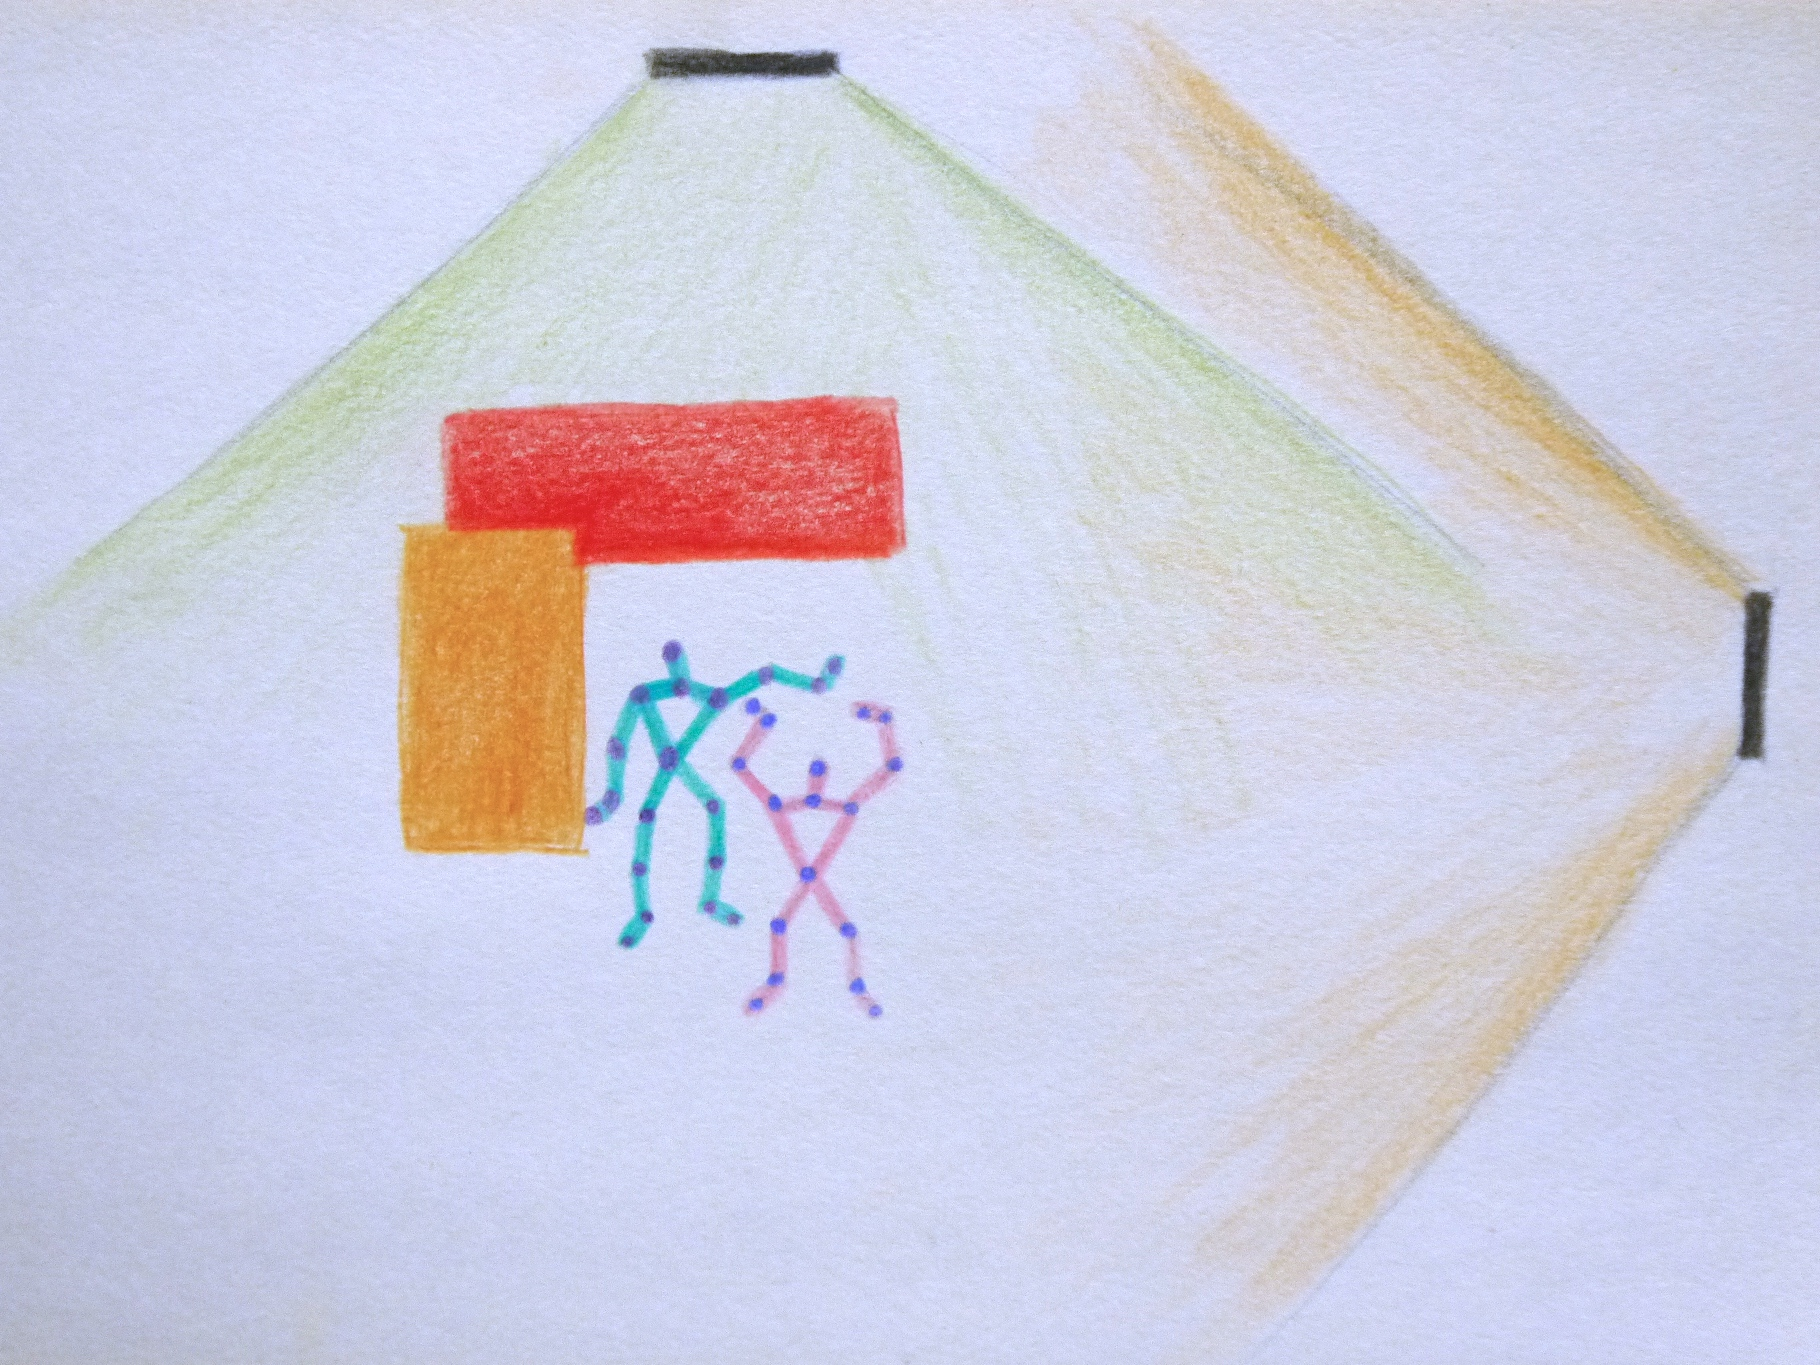
\includegraphics[width=0.5\textwidth]{occlusion_description}
	\caption{The problem of occlusion}
	\label{fig:occlusion_description}
\end{figure}

\section{Background}

Real time detecting and tracking multiple people have been achieved in systems that use RGB-D data\cite{track_rgbd}, shape analysis, stereo and intensity images\cite{w4s}, and appearance-based tracking\cite{track_robust}.

\subsection{Kinect}

Kinect is a low-cost for body motion capturing and tracking. The sensor produces depth and RGB streams at 30 frames per second \cite{kinect_sensor_specs}. It also provides infrared and audio streans. The current work will use Kinect's underlying technology of skeleton detection and tracking. Different components of the Kinect are cater for different tasks. For isntance, the depth stream is useful for tracking people's positions and performing cluster analysis on various objects in the scene. On the other hand, the color information is useful for matching targets in groups of visually different people.

\subsection{Literature Review}


\section{Setup}

The current project is written in C\# and uses the Microsoft Kinect SDK (v.2.0.1410.019000). The current Kinect SDK does not support multiple Kinects on a single machine; as a result, two machines are used for running two Kinects. Machine 1 is the server which runs the tracking algorithm. It has a 2.9 GHz CPU and 8.0 GB RAM. Machine 2 has a 2.3 GHz CPU and 8.0 GB RAM. Both machines runs the Microsoft Windows 8 Operating System, and they stream Kinect frames to the server on Machine 1. The server must start first before running the clients.

\section{Method}

\subsection{Sockets}

TPC soockets are used to transmit serialized Kinect skeleton data from the client to the server.

\subsection{Serialization}

Kinect frames are not serializable by default in the Kinect SDK. A library is written to serialize Kinect data into bytes, which would allow clients to trasnmit them to the server through TPC sockets. The following data are serialized and transmitted:

\begin{itemize}
	\item BodyFrame
		\begin{enumerate}
			\item Timestamp
			\item Depth frame width
			\item Depth frame height
		\end{enumerate}
	\item Body
		\begin{enumerate}
			\item Is tracked
			\item Tracking id
		\end{enumerate}
	\item Joint
	  	\begin{enumerate}
			\item Tracking state
			\item Joint type
			\item Camera space point
			\item Depth space point
			\item Orientation
		\end{enumerate}
\end{itemize}

These data are then deserialized on the server-side. For more information on the data types, visit the Microsoft Kinect documentation [1].

\subsection{Calibration}

The tracking algorithm should calibrate all of the Kinects connected to the server. The process calculates the initial angle and center position of each skeleton with resepct to every Kinect. The initial angle is defined as the angle between the Kinect and the skeleton [INSERT Code Initial Angle]. The center position is defined as the average position of all the joints in the skeleton [INSERT Code Center Position]. These information are essential for converting 3D coordinates in the Kinect camera space to 3D coordinates in the world view coordinate system. This step is the foundation of matching skeletons across different Kinect field of views. Later, the algorithm would match skeletons from different field of views that have the most proximity to each other.

Figure \ref{fig:kinect_camera_space} shows the Kinect camera space. The 3D coordinates (x, y, z) are expressed in meters. The origin of the coordinate system (0, 0, 0) is at the center position of the IR sensor on Kinect \cite{kinect_coordinate_space}. According to the Microsoft specification, the x axis grows to the left of the sensor, the y axis grows upward, and the z axis grows outward from the direction the sensor.

\begin{figure}[H]
	\centering
	
\includegraphics[width=0.5\textwidth]{na}
	\caption{Kinect 3D coordiinate space}
	\label{fig:kinect_camera_space}
\end{figure}

[Describe the worldview coordinate system] \ref{fig:world_view_space}

\begin{figure}[H]
	\centering
	
\includegraphics[width=0.5\textwidth]{na}
	\caption{World view space}
	\label{fig:world_view_space}
\end{figure}

The server synchronizes the calibration process, which is perfomred only once prior to the tracking process. For every Kinect, the algorithm uses the most recent 120 Kinect Body frames, or an equivalent of four seconds, to perform calibration. The server will automatically start the calibration process once it has received sufficient frames from all the clients. The calibration algorithm is taken from [2].

\subsubsection{Initial angle}

\begin{lstlisting}
Calculating initial angle
\end{lstlisting}

\subsubsection{Initial center postion}

\begin{lstlisting}
Calculating initial center position
\end{lstlisting}

\subsubsection{Coordinates in world view}

\begin{lstlisting}
Coordinates transformation
\end{lstlisting}

\subsection{Tracking}

\subsubsection{Matching Skeletons}

\begin{lstlisting}
algorithm pseudocode
\end{lstlisting}

\section{Testing}

The Multiple Kinect UI shows the result of the tracking process (Figure \ref{ui_multiple_Kinects}). The Tracking UI demonstrates (Figure \ref{fig: ui_tracking}) the functionality of converting skeletons into the camera space of any selected Kinect sensor. This shows that the tracking algorithm can accurately match skeletons which follow their respective tracked person, regardless of the reference FOV.


\begin{figure}[H]
	\centering
	
\includegraphics[width=0.5\textwidth]{na}
	\caption{The Multiple Kinect UI showing the result of matching skeletons across different FOVs}
	\label{fig:ui_multiple_Kinects}
\end{figure}

\begin{figure}[H]
	\centering
	
\includegraphics[width=0.5\textwidth]{na}
	\caption{The Multiple Kinect UI showing the functionality of the tracking system}
	\label{fig:ui_tracking}
\end{figure}

\subsection{Without occlusion}

Figure \ref{fig:fov1_all} shows the tracking of one person without occlusion using two Kinects. The left image displays the skeletons of the same person from two difference Kinects' perspective. The right image displays the person's position calculated by the tracking algorithm after matching the skeletons belonging to that person. The skeleton in white color represents the average position of the skeletons from different Kinect FOVs. 

\begin{figure}[H]
	\centering
	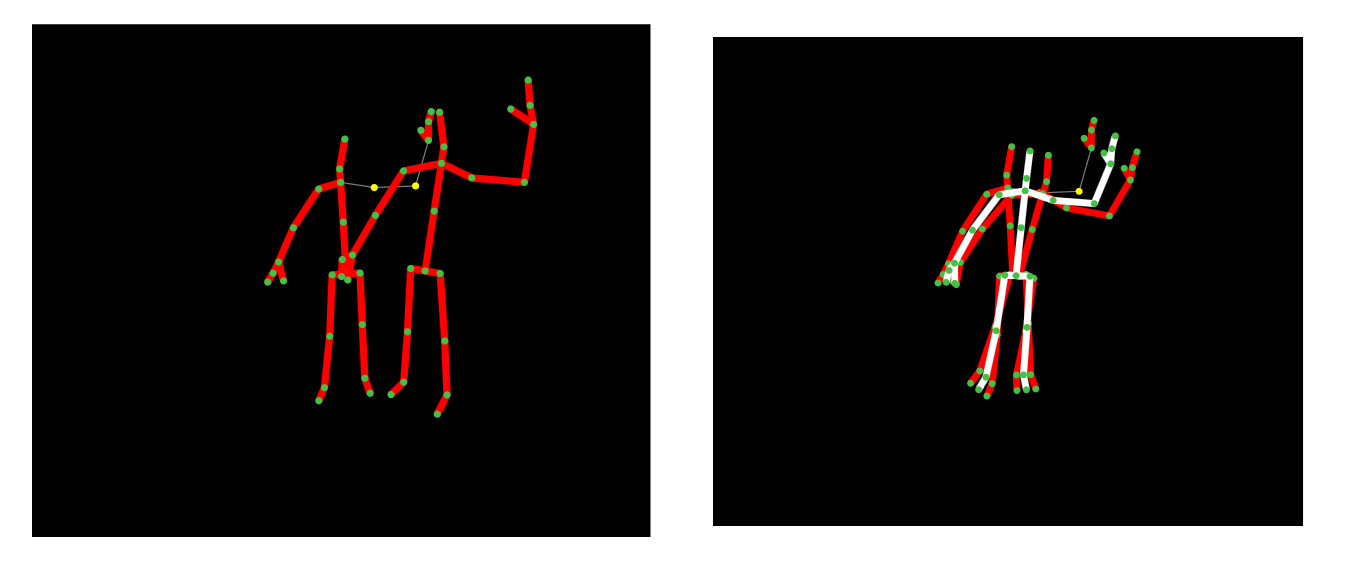
\includegraphics[width=0.5\textwidth]{fov1_all}
	\caption{Tracking of one person with respect to the Kinect FOV of the left skeleton}
	\label{fig:fov1_all}
\end{figure}

\begin{figure}[H]
	\centering
	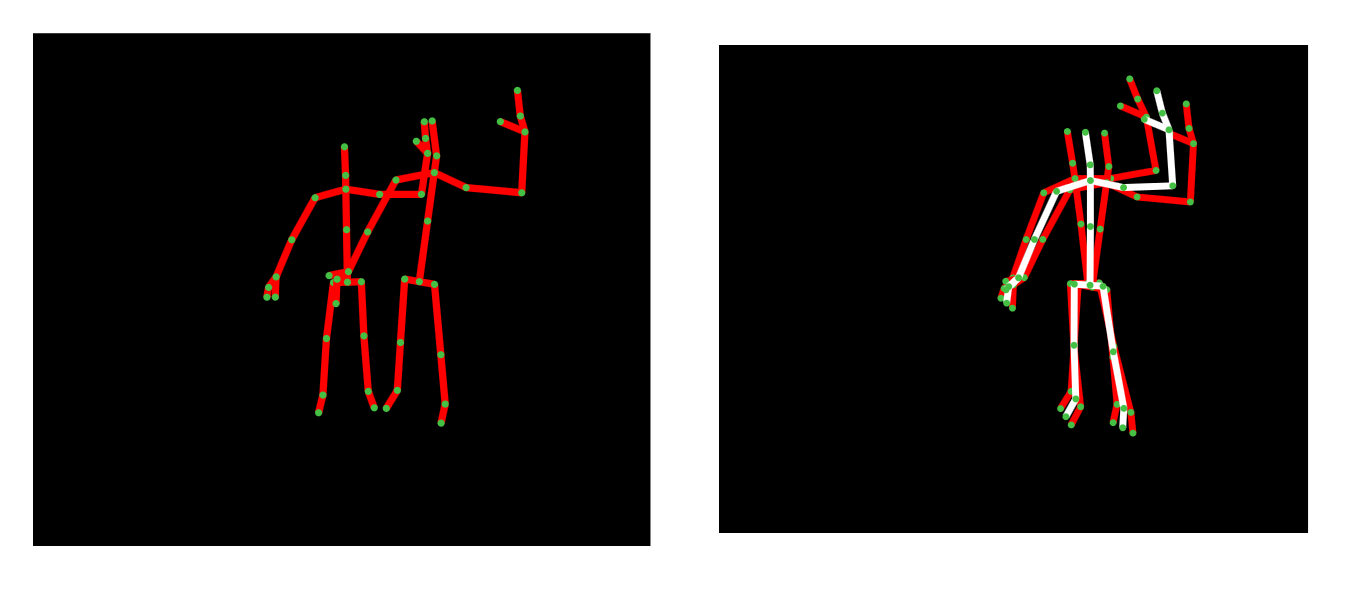
\includegraphics[width=0.5\textwidth]{fov2_all}
	\caption{Tracking of one person with respect to the Kinect FOV of the right skeleton}
	\label{fig:fov2_all}
\end{figure}

\subsection{With occlusion}

\section{Evaluation}

\subsection{Frame rate}



\subsection{Tracking}

The system logs the skeleton coordinates in Kinect camera space for each person with respect to the local Kinect sensor connected to the server machine. The logger writes the coordinates to file every quarter second and flushes the buffer every three seconds. The data are then post-processed to derive each person's average of the skeleton coordinates across different FOVs at every time interval. The differences between the skeleton coordinates from different FOVs and the average are also calculated.

\section{References}
\bibliographystyle{plain}
\bibliography{reportbib}

\end{document}
